\documentclass[fleqn,a4paper,12pt]{article}

%used Packages
\usepackage{standalone}		% Zum Einlesen aus anderen .tex-Files
\usepackage{geometry}		% Zur Bearbeitung des Layouts (Ränder,...)
\usepackage[german]{babel}
\usepackage[utf8]{inputenc}
\usepackage{amsmath}		% Mathematische Symbole
\usepackage{amssymb}     	% Nochmehr mathematische Symbole
\usepackage{dsfont}      	% Schriftsatz fuer Zahlenmengensymbole
%\usepackage{verbatim}   	% erweiterte Verbatim-Umgebung
\usepackage{alltt}       	% Quasi-Verbatim-Umgebung
\usepackage{fancyhdr}    	% Eigene Kopfzeilen
\usepackage{graphicx}    	% Zum Einbinden von Grafiken
							% Einbinden einer eps-Grafik geht so: includegraphics{path}
\usepackage{wrapfig}
\usepackage{lscape}
\usepackage{rotating}
\usepackage{epstopdf}

% Skalierung der Grafiken
\setlength{\unitlength}{1cm}

\frenchspacing               % Kein Extrafreiraum nach Satzzeichen
\setlength{\parindent}{0pt}  % Neue Absaetze nicht einruecken
%\sloppy                     % Schlampige Absatzformatierung
\fussy                       % Penible Absatzformatierung
\linespread{1.5}             % Zeilenabstand


% Seitenraender
\geometry{left=30mm, right=40mm, bottom=30mm}
				% Doc-class, Packageimports, fancy stuff
%Seitenränder formatieren
\addtolength{\voffset}{-2cm}
\addtolength{\textheight}{0cm}
\addtolength{\hoffset}{0cm}
\addtolength{\textwidth}{2cm}
\addtolength{\headheight}{2cm} % fuer jeden Strichkode einen Zentimeter

% Font fuer Code 39
\font\xlix=wlc39 scaled 1200
\newcommand\barcode[1]{{\xlix@#1@}}

% Name, Matrikelnummer, Barcode
\newcommand\student[2]{
	\mbox{\scriptsize
		\begin{tabular}{@{}l@{}r@{}}
			\multicolumn{2}{@{}r@{}}{\barcode{#2}}\\
			#1&#2\\
		\end{tabular}}}

% Kopfzeile
\pagestyle{fancy}            % Eigene Kopfzeilen verwenden
\lhead{
	\small
	\textsc{Grundlagen der Signalverarbeitung \\
		WS 2017/2018 \\
		\"Ubung (\today)}
	\vfill}
\rhead{
	\begin{tabular}[b]{@{}rr@{}}
		\student{Philipp Badenhoop}{572693} &
		\student{Steven Lange}{568733} \\
		\student{Pascal Jochmann}{575056} &
		\student{Kevin Trogant}{572451}
\end{tabular}}			% Definition der Kopfzeile
%andere Definitionen
\providecommand{\R}{{\mathbb R}}
\providecommand{\N}{{\mathbb N}}
\providecommand{\Z}{{\mathbb Z}}
\providecommand{\Q}{{\mathbb Q}}
\providecommand{\C}{{\mathbb C}}
\providecommand{\F}{\mathcal{F}}
\providecommand{\less}{\setminus}
\providecommand{\inv}{{}^{-1}}
\providecommand{\Land}{\bigwedge}
\providecommand{\Lor}{\bigvee}			% Liste der zusätzlichen Commands und redefines

\begin{document}
	\section*{Aufgabe 22}
		Sei $s(t) = \sin(2\pi\cdot t)$ und $c(t) = \cos(2\pi\cdot t)$.\\
		Zwei Funktion $f,g:\R\to\R$ sind auf einem Intervall $[l,r]\subset\R$ orthogonal, wenn $\int_l^rf(x)g(x)dx = 0$ gilt.\\
		\\
		Sei weiter o.B.d.A. $[a,b]\subset \R, a < b$, bel. und $\lambda$ das Standard-Lebesgue-Maß, dann gilt:
		\begin{align*}
			\int_{[a,b]} s(t)c(t)\lambda(dt) =\ & \int_{[a,b]}\sin(2\pi\cdot t)\cos(2\pi\cdot t)\lambda(dt)\\
			=\ & \left[\frac{1}{8\pi}-\frac{\cos(4\pi\cdot t)}{8\pi}\right]_a^b\\
			=\ & \frac{1}{8\pi}-\frac{\cos(4\pi\cdot a)}{8\pi}-\frac{1}{8\pi}+\frac{\cos(4\pi\cdot b)}{8\pi}\\
			=\ & \frac{\cos(4\pi\cdot a) - \cos(4\pi\cdot b)}{8\pi}\overset{!}{=} 0\\
			\Leftrightarrow\ & \cos(4\pi\cdot a) - \cos(4\pi\cdot b) \overset{!}{=} 0\\
			\Leftrightarrow\ & \cos(4\pi\cdot a) \overset{!}{=} \cos(4\pi\cdot b)\\
			\Leftrightarrow\ & \cos(4\pi\cdot a) \overset{!}{=} \cos(4\pi\cdot b + 2k\pi)	& k\in\Z\text{ (Periodizitätseigenschaft)}\\
			\Leftarrow\	& 4\pi \cdot a \overset{!}{=} -4\pi\cdot b - 2k\pi& \cos \text{ (Achsensymmetrie)}\\
			\Leftarrow\	& 4\pi \cdot a \overset{!}{=} 4\pi\cdot \left(-b  -\frac{k}{2}\right)\\
			\Leftrightarrow\ & a \overset{!}{=} -b  -\frac{k}{2}\\
			\Leftrightarrow\ & b \overset{!}{=} -a  -\frac{k}{2}
		\end{align*}
		Das heißt, falls $b = -a  -\frac{k}{2}$ für $k\in\Z$ bel., so ist das Integral
		$$\int_{[a,b]}\sin(2\pi\cdot t)\cos(2\pi\cdot t) \lambda(dt) = 0$$
		auf dem Intervall $[a,b]$.
		Daraus folgt, dass mit
		$$\Gamma := \left\lbrace [a,b]\subset \R \left| a\in\R, k\in\Z: b = -a  -\frac{k}{2} \right.\right\rbrace$$
		gilt 
		$$\forall G\in \Gamma:\int_G\sin(2\pi\cdot t)\cos(2\pi\cdot t) \lambda(dt) = 0.$$
\newpage
	\section*{Aufgabe 23}
		\begin{tabular}{|c|c|c|c|c|c|c|c|c|c|}
			\hline
			$\mathbf{n}$   & 0 & 1 & 2 & 3   & 4 & 5 & 6 & 7 & 8 \\
			\hline
			$\mathbf{t_n}$ & 0 & 1 & 2 & 3   & 4 & 5 & 6 & 7 & 8 \\
			\hline
			$\mathbf{f_n}$ & 1 & 0 & 1 & 1 & 0 & 1 & 1 & 0 & 1\\
			\hline
		\end{tabular} \\
		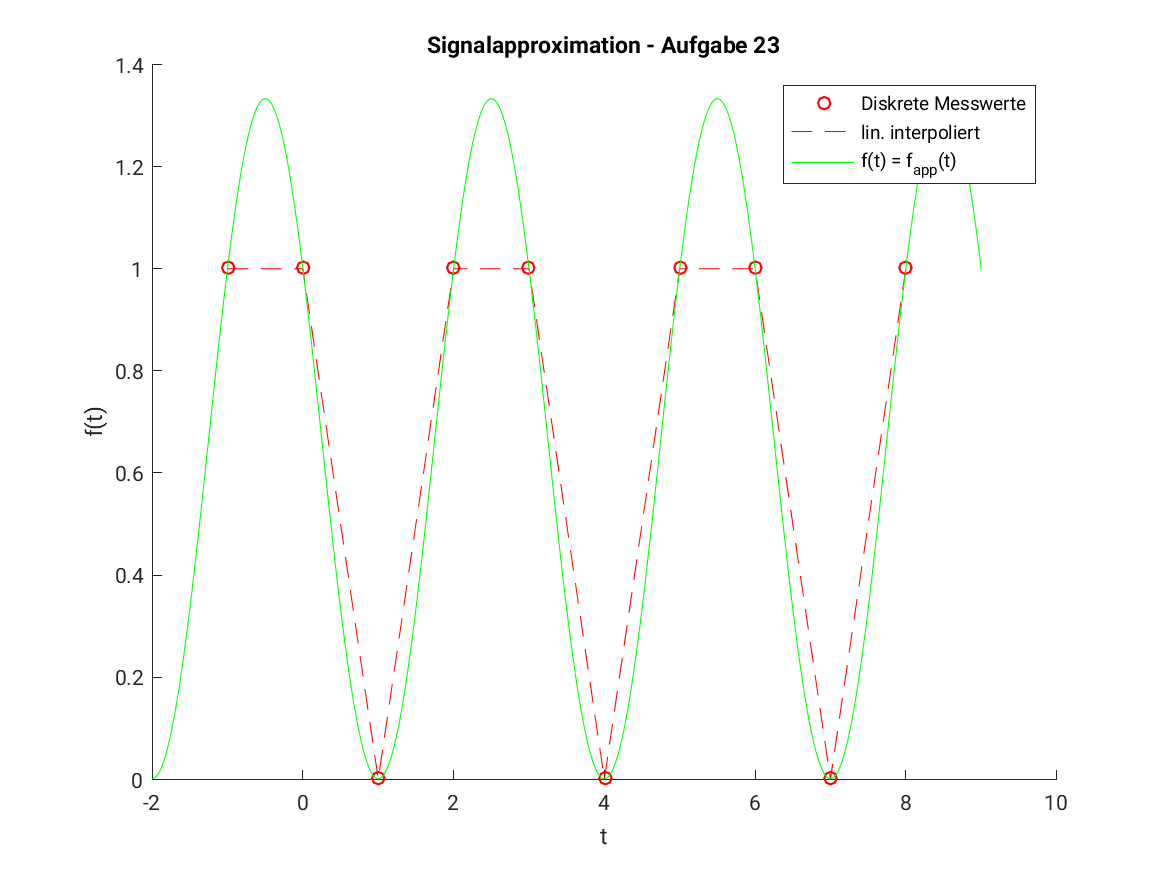
\includegraphics[scale = 0.7]{A23_plot.png}\\
		Aus der Graphik lässt sich die Periodendauer $T_0 = N = 3$ ablesen und die Grundkreisfrequenz $\omega _0 = \frac{2\pi}{N} = \frac{2\pi}{3}$ ableiten.\\
		Sei $f_{app}(t_n) = \frac{a_0}{2} + a_1\cos\left(n\cdot\omega_0\right) + b_1\sin\left(n\cdot\omega_0\right)$ dann gilt für die Koeffizienten
		
		$$a_k = \frac{2}{3}\sum_{n=0}^2f(t_n)\cos\left(kn\cdot \omega_0\right),\quad k\in\{ 0, \dots, 1\}$$
		$$b_k = \frac{2}{3}\sum_{n=0}^2f(t_n)\sin\left(kn\cdot \omega_0\right),\quad k\in\{ 0, \dots, 1\}$$
		
		\begin{tabular}{c | c l}
			$a_0$ & $\frac{4}{3}$			&$= \frac{2}{3}\sum_{n=0}^2f(t_n)\cos\left(0\right)$\\
			$b_0$ & $0$ & \\
			$a_1$ & $\frac{1}{3}$			&$= \frac{2}{3}\sum_{n=0}^2f(t_n)\cos\left(n\cdot \omega_0\right)$\\
			$b_1$ & $-\frac{\sqrt{3}}{3}$	&$= \frac{2}{3}\sum_{n=0}^2f(t_n)\sin\left(n\cdot \omega_0\right)$
		\end{tabular}\\
		\\
		Seien weiter folgende Basisfunktionen gewählt:\\
		$\varphi _0 = 1$, $\varphi _1 = \cos(\omega _0t) = \cos\left(\frac{2\pi t}{3}\right)$ und  $\varphi _2 = \sin(\omega _0t) = \sin\left(\frac{2\pi t}{3}\right)$\\
		Dann gilt:
		$f_{app}(t) = \frac{2}{3}\varphi_0 + \frac{1}{3}\varphi_1 - \frac{\sqrt{3}}{3}\varphi_2 \approx 0.667 + 0.333\cdot \cos\left(\frac{2\pi t}{3}\right) - 0.577\cdot \sin\left(\frac{2\pi t}{3}\right)$\\
		$e^2$ ist genau 0, weil die Anzahl der Messwerte in einer einzelnen Periodendauern N genau gleich der Anzahl der Basisfunktionen m ist (beides = 3).\\
		\\
		Aus der gegebenen Tabelle lassen sich nun die komplexen Koeffizienten berechnen: $c_0 = 0.667$ sowie $c_1 = 0.167 + j\cdot 0.289$ und $c_1^* = 0.167 - j\cdot 0.289$.\\
\end{document}